\newpage
\section{Convessità}
\subsection{Funzione convessa}
\begin{definition}[Convessa]
Dato un $I \subset \mathbb{R}$ intervallo\footnote{Si parla sempre di intervalli quando si parla di convessità perché la convessità non ha senso sennò} ed una $f: I \to \mathbb{R}$. $f$ si dice \textbf{convessa} in I se, presi due punti qualsiasi sul grafico di $f$ il segmento che li unisce è sopra il grafico di $f$.
\end{definition}
\begin{wrapfigure}[6]{r}{6cm}
    \vspace{-10pt}
    \centering
    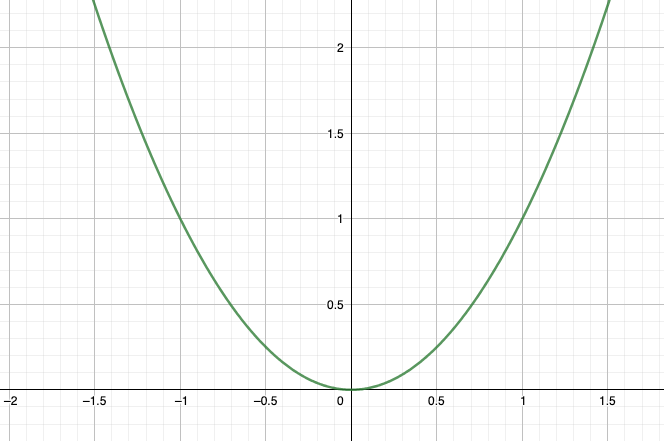
\includegraphics[width=3.8cm]{images/convessa.png}
    \caption{Funzione convessa}
\end{wrapfigure}
\hspace{-15pt}In formule si esprime dicendo che: $f$ si dice convessa in $I$ se $\forall x_1, x_2 \in I$ con $x_1 < x_2$ e $\forall t \in (0,1)$ risulta che:
\begin{center}
    $f(x_1 + t(x_2 - x_1)) \leq f(x_1) + t(f(x_2) - f(x_1))$
\end{center}
Se la stessa disuguaglianza vale con il $<$ (minore stretto) allora $f$ si dice strettamente convessa.

\subsection{Funzione concava}
\begin{definition}[Concava]
$f$ si dice concava se $-f$ è convessa. Strettamente concava se $-f$ è strettamente convessa.
\end{definition}
\begin{wrapfigure}[6]{l}{6cm}
    \vspace{-10pt}
    \centering
    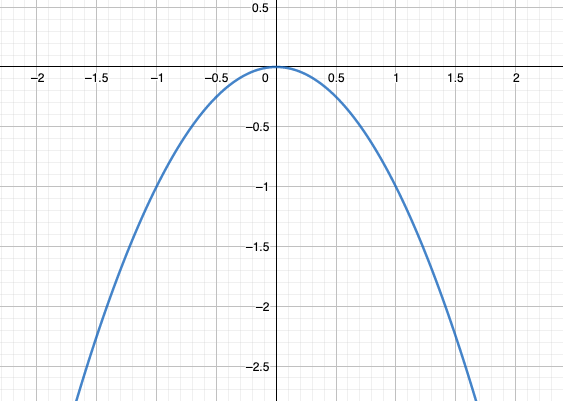
\includegraphics[width=3.8cm]{images/concava.png}
    \caption{Funzione concava}
\end{wrapfigure}
Se andiamo a scrivere in formule una funzione concava è uguale a:
\begin{center}
    $f(x_1 + t(x_2 - x_1)) \geq f(x_1) + t(f(x_2) - f(x_1))$
\end{center}
\begin{note}
Nota che, come per la concavità, se andiamo scrivere $>$ (maggiore stretto) allora $f$ si dice strettamente concava.
\end{note}

\vspace{15pt}
\subsection{Calcolo della convessità}
\begin{proposition}
Dato $I \subset \mathbb{R}$ intervallo, $f: I \to \mathbb{R}$ derivabile 2 volte. Sono equivalenti:
\begin{enumerate}
    \item $f$ è convessa (strettamente convessa).
    \item $f'$ è debolmente crescente (strettamente crescente).
    \item $f'' \geq 0$ ($f'' > 0$).
\end{enumerate}
\end{proposition}

\begin{note}
La proposizione è uguale per la concavità ma con il segno scambiato.
\end{note}

\begin{example}
$f(x) = x^2$ da $f:\mathbb{R} \to \mathbb{R}$.\\
$f'8x) = 2x$, $f''(x) = 2 > 0 \: \forall x \in \mathbb{R} \Longrightarrow f$ è convessa (anche strettamente) in tutto $\mathbb{R}$.
\end{example}

\begin{example}
$f(x) = e^x$ e $f'(x) = e^x$, $f''(x) = e^x > 0$ sempre $\Longrightarrow f:\mathbb{R} \to \mathbb{R}$ è strettamente convessa.
\end{example}

\begin{example}
$f(x) = \log(x)$ con $f:(0,+\infty) \to \mathbb{R}$.\\
$f'(x) = \frac{1}{x}$, $f''(x) = \frac{1}{x^2} < 0 \: \forall x > 0 \Longrightarrow f$ è strettamente concava. 
\end{example}

\subsection{Interpretazione geometrica}
\begin{wrapfigure}[7]{l}{6cm}
    \vspace{-13pt}
    \centering
    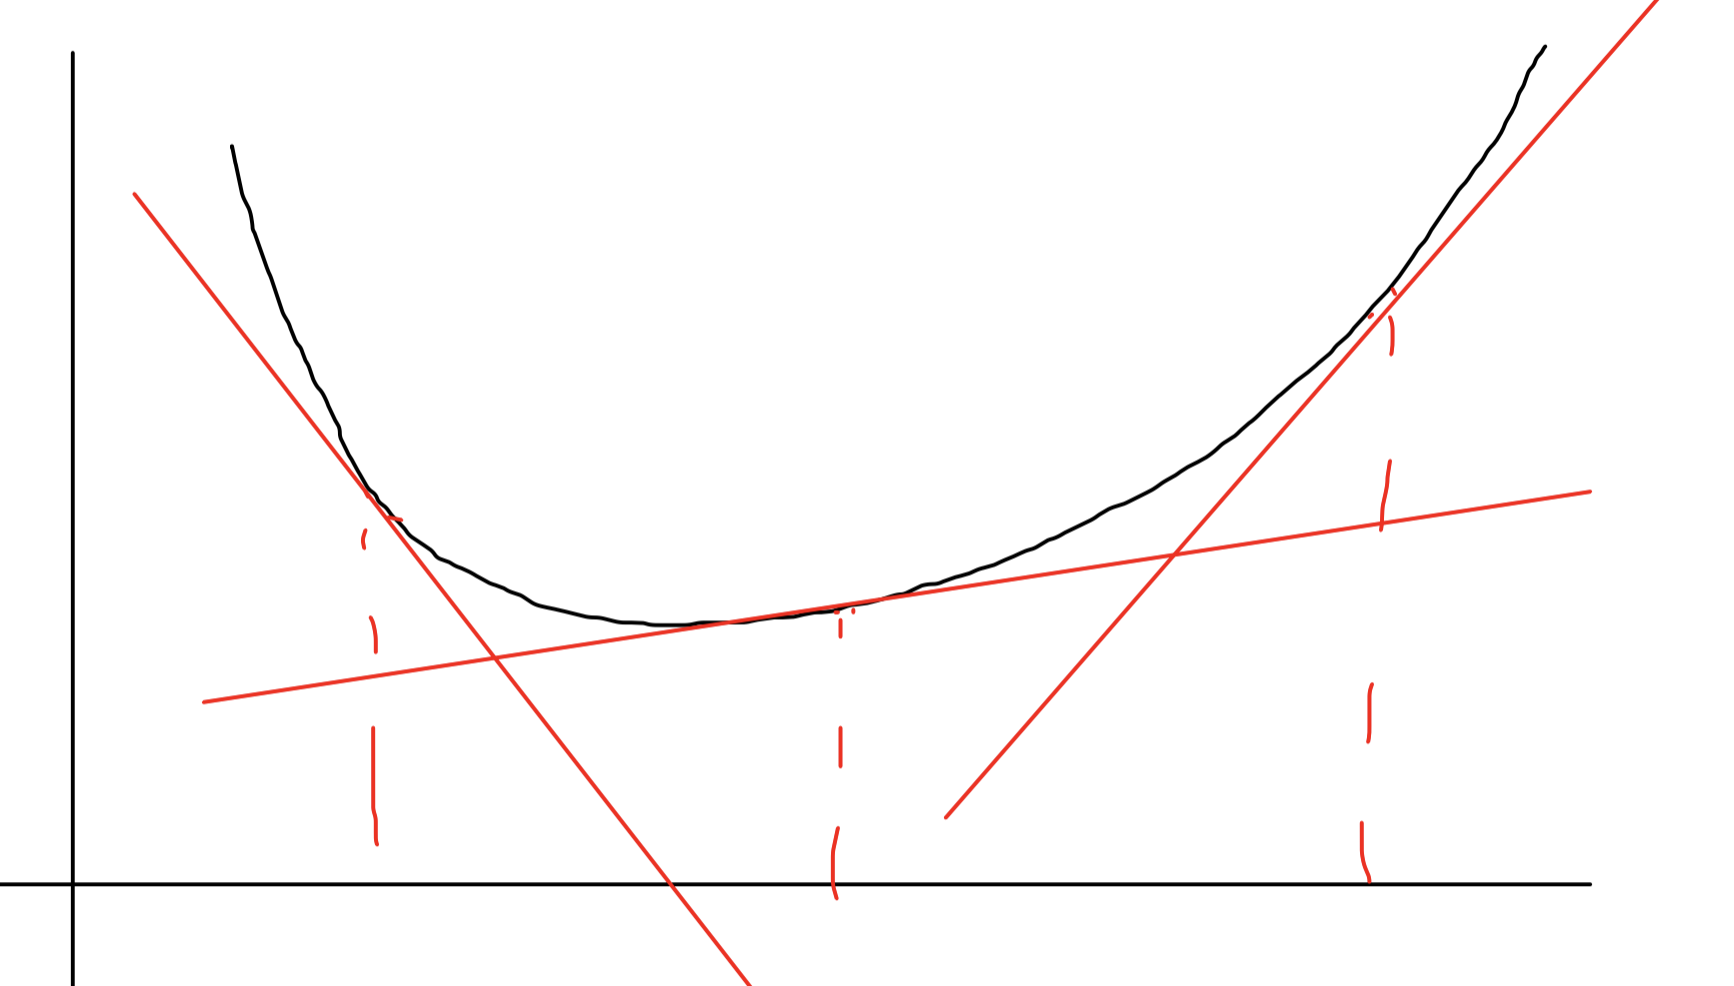
\includegraphics[width=5.5cm]{images/interpretazione-geometrica-convessita.png}
\end{wrapfigure}
Dire che $f'$ è crescente vuol dire che diciamo che il coefficiente angolare sulla tangente cresce, e questo vuol dire che se noi pensiamo alla retta tangente come un punto che tocca il grafico e mano a mano si sposta sul grafico e così facendo va a cambiare inclinazione ruotando, quindi possiamo dire che "la tangente ruota in senso antiorario".\\
\newpage
\begin{example}
Esempio di funzione concava e convessa solo in sotto intervalli del dominio.
\end{example}
\begin{wrapfigure}[4]{r}{8cm}
    \vspace{-10pt}
    \centering
    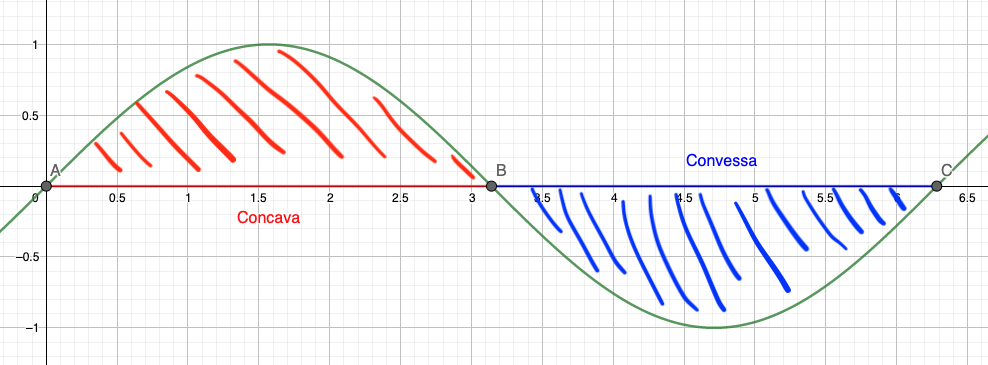
\includegraphics[width=7cm]{images/seno-concavo-convesso.png}
\end{wrapfigure}

$f(x) = \sin{x}$, $f: [0, 2\pi]$. $f'(x) = \cos{x}$ e $f''(x) = -\sin{x}$.\\
$-\sin{x} \geq 0. \Longleftrightarrow \sin{x} \leq 0 \Longleftrightarrow x \in [\pi, 2\pi]$.\\
$f''(x) \geq 0 \Longleftrightarrow x \in [\pi, 2\pi]$ \hspace{.5cm} $f''(x) \leq 0 \Longleftrightarrow x \in [0, \pi]$\\\\

\begin{proposition}
Prendiamo un $I \subset \mathbb{R}$ intervallo, una $f: I \to \mathbb{R}$ derivabile. Allora $f$ è convessa in $I$ se e solo se $\forall \: x_0 \in I$ il grafico di $f$ è sopra la retta tangente nel punto $(x_0, f(x_0))$ cioè, $\forall \: x_0, x\in I$:
\[f(x) \geq f(x_0) + f'(x_0)(x-x_0)\]
Concava se vale il $\leq$. Stret. convessa se vale $>$ con $x \neq x_0$ e stret. concava se vale $<$ con $x\neq x_0$.
\end{proposition}

\begin{note}
Il grafico  di $f(x_0) + f'(x_0)(x-x_0)$ è la retta tangente.
\end{note}

\begin{example}
$f(x) = e^{-|x|}$, questa è una funzione pari e $f(x) = e^{-x}$ se $x \geq 0$.\\
Questa funzione non è ne concava ne convessa in tutto $\mathbb{R}$, perché ci sono dei tratti dove $f$ sta sotto altri dove sta sopra.\\\\
$f(x) = e^{-|x|} = \begin{cases}e^{-x} & \text{ se } x\geq 0\\e^{x} & \text{ se } x < 0\end{cases}$ \\\\
Quindi se $x>0$ $f'(x) = -e^{-x}$ e $f''(x) = e^{-x} > 0 \Longrightarrow f$ è convessa sull'insieme $\{x>0\}.$\\
Mentre se $x<0$ $f'(x) = e^{-x}$ e $f''(x) = e^{x} > 0 \Longrightarrow f$ è convessa sull'insieme $\{x\leq0\}.$
\end{example}
\hspace{-15pt}Da questo esempio vediamo che se prendiamo $f$ in due intervalli separati, in entrambi questi intervalli è convessa ma nell'unione dei due intervalli $f$ smette di essere convessa. Il motivo è che abbiamo un punto in $x=0$ di non derivabilità.

\begin{example}
Se invece prendiamo $f(x) = e^{|x|}$ quindi $f(x) = \begin{cases}e^x & \text{ se } x\geq 0 \\e^{-x} & \text{ se } x< 0 \end{cases}$.\\\\
In questo caso $f$ è convessa in $(-\infty, 0]$ ed è convessa anche in $[0, +\infty)$ e in questo caso $f$ è convessa anche in tutto $\mathbb{R}$.
\end{example}

\hspace{-15pt}Possiamo notare che nel secondo esempio se calcoliamo $f'_-(0) = -1$ e $f'_+(0) = 1$ mentre se vediamo l'esempio prima $f'_-(0) = 1$ e $f'_+(0) = -1$.

\begin{proposition}
Prendiamo un $I \subset \mathbb{R}$ intervallo, $x_0$ punto interno di $I$, $f:\mathbb{R} \to \mathbb{R}$ derivabile in $I \setminus \{x_0\}$. Siano $I_1 = \{x \in I \: |\: x<x_0\}$ e $I_2 = \{x\in I \: |\: x > x_0\}$ abbiamo che se $f$ è convessa in $I_1$ e $I_2$ e $x_0$ è un punto angoloso per $f$ allora $f$ è convessa in $I$ se e solo se $f'_-(x_0) \leq f'_+(x_0)$.
\end{proposition}

\hspace{-15pt}Questa cosa perché, se noi prendiamo una funzione che presenta un angolo e tracciamo la tangente, data dalla derivata, a sinistra notiamo che mano a mano che ci spostiamo verso destra questa tangente "ruoterà" sul grafico, nel punto $x_0$ avremo due tangenti una dalla derivata destra ed una dalla sinistra, possiamo notare che se la funzione rimane concava o convessa questa tangente continuerà a "ruotare" nello stesso verso senza fare "uno scatto" nel suo andamento, in caso contrario allora non manterrà la concavità o la convessità.

\subsection{Flessi}
\begin{definition}[Flesso]
Dato un $I\subset \mathbb{R}$ intervallo, $f: I\to \mathbb{R}$, $x_0$ punto interno ad $I$ si dice punto di flesso se $f$ è derivabile in $x_0$ ed esiste un intorno $U \subset I$ di $x_0$ t.c. la quantità
\[\frac{f(x) - (f(x_0) + f'(x_0)(x-x_0))}{x-x_0} \text{ non cambia segno in }U \setminus \{x_0\}\]
\end{definition}

\hspace{-15pt}Dire che $\frac{f(x) - (f(x_0) + f'(x_0)(x-x_0))}{x-x_0}$ non cambia segno vuol dire che il grafico della funzione passa da sopra a sotto la tangente (o viceversa).

\begin{definition}[Flesso a tangente verticale]
Se invece $f'(x) = \pm\infty$ ($f$ non è derivabile), $f$ è continua in $x_0$, e se $f$ è convessa in un intorno destro di $x_0$ e concava in un intorno sinistro di $x_0$ (o viceversa) allora $x_0$ si dice punto di flesso a tangente verticale. 
\end{definition}

\hspace{-15pt}Un flesso verticale è un cambiamento di convessità con un flesso verticale.

\begin{observation}
Se avete una funzione $f: I \to \mathbb{R}$, $I$ intervallo ed $f$ derivabile due volte in $I$. Allora se $f''(x_0)=0$ e $f$ cambia segno in $x_0$ allora $x_0$ è punto di flesso.
\end{observation}

\hspace{-15pt}Cambia segno vuol dire che $f''(x) \leq 0$ se $x\leq x_0$ e $f''(x) \geq 0$ se $x\geq x_0$ (o viceversa), con $x \in U$ intorno di $x_0$.

\begin{example}
Calcoliamo il flesso di $f(x) = x^3$, $f'(x) = 3x^2$, $f''(x) =6x$.\\
Vediamo dall'immagine che esiste un flesso in $x=0$, infatti:\\
$f''(x) = 0$, $f''(x) \leq 0$ se $x \leq 0$ e $f''(x) \geq 0$ se $x \geq 0$.
\end{example}

\begin{observation}
$f''(x_0) = 0$ non è sufficiente per aver un flesso
\end{observation}

\begin{example}
Prendiamo per verificare l'osservazione $f(x) = x^4$, $f'(x) = 4x^3$, $f''(x) = 12x^2$.\\
Anche se $f(0)=0$ abbiamo che $f''(x) \geq 0 \forall x \in \mathbb{R} \Longrightarrow $ f è convessa in $\mathbb{R}$.
\end{example}

\begin{observation}
Ci possono essere punti di flesso dove non esiste la derivata seconda.
\end{observation}

\begin{example}
$f(x) = x \cdot |x|$\hspace{.3cm} $f(x) = \begin{cases}x^2 & \text{ se } x \geq 0\\ -x^2 & \text{ se } x<0\end{cases}$\hspace{.3cm} $f'(x) = \begin{cases}2x & \text{ se } x>0 \\ -2x & \text{ se } x<0\end{cases}$\\\\
Possiamo vedere che $x_0 = 0$ è punto di flesso, infatti $f$ è derivabile in $x_0 = 0$ infatti $f'(0) = \lim\limits_{x\to 0}\frac{f(x) - f(0)}{x-0} = \lim\limits_{x\to 0}|x| = 0$.
La retta tangente in $x=0$ è $y=0$. $f$ passa da sopra la tangente in $x_0 = 0$, quindi $x_0$ è un punto di flesso. Però non esiste la derivata seconda in $x_0 = 0$ perché in questo punto c'è un punto angoloso.
\end{example}

\begin{observation}
Se abbiamo una funzione $f: I \to \mathbb{R}$, con $I \subset \mathbb{R}$, $f$ convessa nei punti interni di $I$, ed $f$ continua in tutto $I \Longrightarrow f$ è convessa in $I$.\\
Quindi se abbiamo $f:[a,b] \to \mathbb{R}$ convessa in $(a,b)$ ed $f$ continua in $[a,b] \Longrightarrow f$ è convessa in $[a,b]$.
\end{observation}

\newpage
\section{Studio di funzione}
\subsection{Punti da seguire}
Data una funzione $f(x)$ bisogna andare ad eseguire una serie di passi. $f(x)$ viene di solito assegnata senza specificare il dominio.
\begin{enumerate}
    \item Determinare l'insieme di definizione di $f$.
    \item Determinare l'insieme di continuità di $f$.
    \item Determinare l'insieme di derivabilità di $f$.
    \item Vedere eventuali asintoti orizzontali, verticali o obliqui.
    \item Studiare la monotonia della funzione.
    \item Trovare punti di massimo o di minimo locali.
    \item Determinare massimo e minimo d $f$ oppure estremo sup. ed inf.
    \item Studiare la convessità di $f$ (con eventuali punti di flesso).
\end{enumerate}

\subsection{Esempio studio di funzione}
\begin{example}
Studiamo la funzione $f(x) = \log|x| - \frac{x^2 - 1}{4x}$.
\begin{enumerate}
    \item $|x| > 0 \Longleftrightarrow x\neq 0$ e $4x \neq 0 \longleftarrow x \neq 0$. \textbf{Insieme di definizione} è $\mathbb{R} \setminus \{0\}$.
    \item La $f$ è \textbf{continua} in tutto $\mathbb{R} \setminus \{0\}$ (composizione funzioni continue e prodotto e sottrazioni funzioni continue).
    \item $f$ \textbf{derivabile} in tutto $\mathbb{R} \setminus \{0\}$ (sempre perché tutte queste funzioni sono derivabili in tutto il loro insieme di definizione, il valore assoluto non è derivabile in 0 ma non lo si considera).
    \item Per vedere gli \textbf{asintoti} dobbiamo fare i limiti ai bordo e sui punti non interi al dominio:\\
    $\lim\limits_{x\to -\infty}f(x) = \log|x| - \frac{x^2 -1}{4x} = \log|x| - \frac{x}{4} + \frac{1}{4x}$ \hspace{.5cm} $\lim\limits_{x\to -\infty}\log|-\infty| - \frac{-\infty}{4} + \frac{1}{4(-\infty)} = + \infty$.\\
    $\lim\limits_{x\to 0^-}\log|0^-| - \frac{0^-}{4} + \frac{1}{4(0^-)} = -\infty - 0 - \infty$. \hspace{.5cm} 
    $\lim\limits_{x\to 0^+}\log|0^+| - \frac{0^+}{4} + \frac{1}{4(0^+)} = -\infty - 0 + \infty$\\
    $\lim\limits_{x\to 0^+}f(x) = \lim\limits_{x\to 0^+}(-\frac{x}{4}) + \lim\limits_{x\to 0^+}\log|x| + \frac{1}{4x} = 0 + \lim\limits_{x\to 0^+}\frac{4x\log|x| + 1}{4x} = 0 + \frac{0+1}{4 \cdot 0^+} = +\infty$\\
    $\lim\limits_{x\to +\infty} \log|+\infty| - \frac{\infty}{4} + \frac{1}{4 \cdot \infty} = \infty - \infty + 0$\\
    $\lim\limits_{x\to +\infty} x(\frac{\log|x|}{4} - \frac{1}{4}) + \lim\limits_{x\to +\infty} \frac{1}{4x} = \infty(0 - \frac{1}{4}) + 0 = -\infty.$
    Abbiamo quindi un asintoto verticale di equazione $x=0$ e non ci sono asintoti orizzontali. Vediamo se ci sono asintoti obliqui:
    $\lim\limits_{x\to +\infty}\frac{f(x)}{x} = \lim\limits_{x\to +\infty}(\log|x| -\frac{x}{4} + \frac{1}{4x}) \cdot \frac{1}{x} = 0 - \frac{1}{4} + 0 = -\frac{1}{4}$, quindi $m= -\frac{1}{4}$\\
    $\lim\limits_{x\to +\infty}f(x) -mx = \lim\limits_{x\to +\infty} \log|x| - \frac{x}{4} + \frac{1}{4x} + \frac{1}{4}\cdot x = \infty + 0 = \infty$. \\
    Non c'è asintoto obliquo per $x\to +\infty$ e neanche a $x\to -\infty$ perché i conti sono uguali.
    \item Studiamo ora la \textbf{monotonia} di $f$.
    
    $\log|x| = \begin{cases}\log(x) & \text{ se } x>0 \\ \log(-x) & \text{ se } x<0\end{cases}$\hfill
    $D(\log|x|) = \begin{cases}D(\log(x)) = \frac{1}{x} & \text{ se } x>0 \\D(\log(-x)) = \frac{1}{-x} \cdot (-1) = \frac{1}{x} & \text{ se } x<0\end{cases}$
    
    Quindi possiamo notare che $D(\log |x|) = \frac{1}{x}$.\\
    $f(x) = \log|x| - \frac{x}{4} + \frac{1}{4x}$ \hspace{.3cm} $f'(x) = \frac{1}{x} - \frac{1}{4} -\frac{1}{4x^2} = \frac{-x^2 + 4x -1}{4x^2}$ conferma che è derivabile ovunque tranne che in $x = 0$.\\\\
    Il denominatore è $> 0$ in tutto il dominio, allora il segno di $f'$ è lo sesso del numeratore. Per trovare il segno bisogna trovare dove si annulla il numeratore.\\
    $-x^2 + 4x - 1 = 0 \Longleftrightarrow x^2 - 4x + 1 = 0$ \hspace{.3cm} $x = 2 \pm \sqrt{4-1} = 2 \pm \sqrt{3}$.\\
    $f$ è decrescente in $(-\infty,0)$, decrescente in $(0,2-\sqrt{3}]$, crescente in $[2-\sqrt{3}, 2+\sqrt{3}]$, decrescente in $[2+\sqrt{3},+\infty)$. Questa separazione va fatta perché il teorema di Lagrange prevede intervalli e lo 0 interrompeva l'intervallo.
    \item Vedendo la monotonia possiamo anche dire i punti di \textbf{massimo e minimo locali}. \\
    $x = 2 - \sqrt{3}$ è punti di minimo locale. \hspace{.3cm} $x = 2 + \sqrt{3}$ è punti di massimo locale.\\
    Per calcolare esattamente questi punti dove si collocano nel grafico basta sostituirli in $f(x)$.
    \item Dal fatto che $\lim\limits_{x\to +\infty} = +\infty$ otteniamo che $sup(f) = +\infty \Longrightarrow f$ non ha \textbf{massimo}. Dal fatto che $\lim\limits_{x\to 0^-}=-\infty$ otteniamo che $inf(f) = -\infty \Longrightarrow f$ non ah \textbf{minimo}.
    \item Come ultima calcoliamo al derivata seconda e troviamo la \textbf{convessità}.\\
    $f'(x) = \frac{1}{x} - \frac{1}{4} - \frac{1}{4x^2}$ \hspace{.5cm} $f''(x) = -\frac{1}{x^2} +\frac{1}{2x^3} = \frac{-2x + 1}{2x^2}$\\
    Segno del numeratore $-2x + 1 > 0 \Longleftrightarrow 1 > 2x \Longleftrightarrow x < \frac{1}{2}$.\\
    Segno del denominatore $2x^3 > 0 \Longleftrightarrow x > 0$.\\
    $f$ è concava in $(-\infty, 0)$ \hspace{.3cm} convessa in $(0,\frac{1}{2}]$ \hspace{.3cm} concava in $[\frac{1}{2},
    +\infty)$.\\
    Il punti di ascissa $x=\frac{1}{2}$ è punto di flesso visto che c'è un cambio di convessità.
\end{enumerate}
\end{example}